\documentclass[a4paper, 11pt, twocolumn]{article}
\usepackage[utf8]{inputenc}
\usepackage{graphicx}
\usepackage[T1]{fontenc}
\usepackage[ngerman]{babel}
\usepackage{graphicx} 
\usepackage{layout} 
%\usepackage{mathpazo} % Palatino
%\usepackage{helvet} % Helvetica
\usepackage{newcent} % New Century Schoolbook
%\usepackage{courier} % Courier
%\usepackage{mathptmx} % Times New Roman
\usepackage{geometry}
\usepackage{subfigure}
\usepackage{fancyhdr}
\usepackage{expdlist}
\usepackage{makeidx}
\usepackage{tabularx}
\usepackage{multirow}
\usepackage{amsmath,amssymb,amstext}

\fancyfoot[C]{\thepage}%  Spezielle Fusszeile
\begin{document}

\title{\textbf{Tracking von Gesichtern in belebten Umgebungen mit Hilfe eines Partikelfilters}}
\author{ \textit{Kai Wolf} \\ Kai.B.Wolf@student.hs-rm.de\vspace{0.8cm}\\Hochschule RheinMain\\University of Applied Sciences\\Wiesbaden Rüsselsheim Geisenheim}
\date{\today\\[5mm]
\begin{center}
\textbf{Zusammenfassung}\\[2mm]
\begin{minipage}{0.9\textwidth}
Dieses Projekt ist im Rahmen der Vertiefungsveranstaltung Machine Learning im Masterstudiengang Informatik an der Hochschule RheinMain entstanden. Die Veranstaltung fand im Sommersemester 2012 statt und wurde von Prof. Dr. Schwanecke betreut. Die vorliegende Arbeit behandelt das automatisierte Tracking von Personen in einem Videobild anhand des Gesichts in belebten Umgebungen. Mit Hilfe eines Partikelfilters werden anschließend die zuvor klassifizierten Personen über mehrere Frames hinweg verfolgt. Der Quelltext zu dieser Arbeit basiert weitestgehend auf der Veröffentlichung aus dem Jahr 2009~\cite{aliMultipleHuman}.
\end{minipage}
\end{center}
} 
\maketitle

\section{Einleitung} % (fold)
\label{sec:einleitung}
Das automatisierte Tracking von Personen in einem Videobild ist eine anspruchsvolle Aufgabe aus den Bereichen Machine Learning und Computer Vision. Dabei müssen gleich mehrere Problemstellungen gelöst werden: die erfolgreiche Erkennung von Personen im Videobild, die Verfolgung der zuvor entdeckten Personen über mehrere Frames hinweg und schließlich die Anpassung der Verfolgung unter Einbeziehung des Verhaltens der Person~\cite{Yilmaz2006}. 
Des Weiteren spielt die ausreichende Beleuchtung der Umgebung (Tag-/Nachtzeit) eine wichtige Rolle für die stabile Erkennung.
Das Gesicht einer Person ist im Allgemeinen ein stabiles Feature für die Wiedererkennung~\cite{ViolaRobustObject2001}. Dennoch können bei der Detektion gleich mehrere Probleme auftreten: 
Zum einen kann die Erkennung von Gesichtern aufgrund von Schatten oder starken Reflektionen beeinträchtigt werden, zum anderen können Gesichter gerade in belebten Umgebungen wie Straßen oder Fußgängerzonen durch andere Menschen oder Gebäude teilweise oder ganz verdeckt werden~\cite{aliMultipleHuman}. Dabei steigt die Verdeckung durch andere Personen naturgemäß mit der Anzahl an Personen, die gleichzeitig im Videobild zu sehen sind.
Als Lösungsstrategie verwendet die vorliegende Arbeit daher einen bereits trainierten und robusten Viola-Jones-Klassifikator zur Erkennung von Gesichtern und benutzt ein sogenanntes \emph{confirmation-by-classification} Verfahren, um in jedem neuen Frame des Videos erneut nach Gesichtern zu suchen~\cite{aliMultipleHuman}. Dadurch soll die Erkennung insgesamt stabiler und Fehlklassifikationen wie Taschen, Jacken oder Schilder auf ein Minimum reduziert werden. 
Für jede erfolgreiche Klassifizierung einer Person wird anschließend ein Bewegungspfad initialisiert, der die Bewegung der Person mit Hilfe eines Partikelfilters über mehrere Frames hinweg verfolgt. Durch das zuvor erwähnte \emph{confirmation-by-classification} Verfahren und dem Partikelfilter wird bei kurzzeitiger teilweiser bzw. kompletter Verdeckung einer getrackten Person verhindert, dass der Bewegungspfad sofort abreißt, indem in einem Umkreis rund um die letzte entdeckte Region weiter nach der verloren gegangenen Person gesucht wird.
Für eine experimentelle Auswertung wurde ein Video mit einer Auflösung von 480x272 Pixeln verwendet. Das Video wurde in der Münchener Fußgängerzone aufgenommen. Auf der verwendeten Hardware (2,4 GHz Intel Core i5 Prozessor, 8GB RAM) benötigte die verwendete Implementierung ca. 500ms für die Verarbeitung eines Frames. Insgesamt liefen 48 verschiedene Personen durch das Bild. Die Trefferquote lag bei 81.25\%. 

% section einleitung (end)

\section{Bisherige Arbeiten} % (fold)
\label{sec:bisherige_arbeiten}

Für das automatisierte Tracking von Personen in einem Videobild existieren verschiedene Ansätze, die das Tracking von Personen über ein Bewegungsmodel realisieren. 
In der Arbeit von~\cite{zhaoSegmentationTracking} wird die Bewegung einer Person anhand des starr bleibenden Hintergrunds detektiert. In der Veröffentlichung von~\cite{Zhao2004} werden Personen anhand ihrer Körperform identifiziert und die Tatsache genutzt, dass diese (meist) auf einer Ebene durch das Videobild laufen. Eine etwas ältere Arbeit aus dem Jahr 2001 identifiziert Objekte anhand ihrer Features, die zusammengenommen, in nachfolgenden Frames wiedergefunden werden können~\cite{Veenman2001}.

Alle diese Verfahren funktionieren jedoch bei steigender Anzahl von Personen im Videobild nicht mehr richtig, da dadurch die gesamte Szene in Bewegung gerät oder viele Personen im Bild durch andere Personen oder Gegenstände teilweise oder komplett verdeckt werden. Unter diesen Bedingungen stellt das Gesicht einer Person das einzige Feature dar, das in einem Videobild stabil wiedererkannt werden kann~\cite{aliMultipleHuman}.

% section bisherige_arbeiten (end)

\section{Statistische Filter} % (fold)
\label{sec:statistische_filter}

Die sog. Klasse der \emph{statistischen Filter} zeichnet sich durch drei Besonderheiten aus: Statistische Filter fassen Messwerte als Wahrscheinlichkeitsverteilungen auf. Gegenüber der traditionellen Statistik, in welcher die Wahrscheinlichkeit als Sicherheit bzw. Unsicherheit über des Eintreten eines Ereignisses eines Zufallsexperiments definiert ist, benötigen statistische Filter kein Zufallsexperiment als Grundlage. 
Des Weiteren werden immer bedingte Wahrscheinlichkeiten der Form $P(B|A)$ betrachtet. Das bedeutet, es wird die Wahrscheinlichkeit geschätzt, wie plausibel es ist, dass Aussage B eintritt, unter der Voraussetzung, dass A eingetreten ist. Die Berechnung erfolgt mit Hilfe des \emph{Satz von Bayes}~\cite{PapulaFormelsammlung2001}:
\[
	P(B|A) = \frac{P(A \cap B)}{P(A)}
\]
Die dritte Besonderheit ist, dass unbekannte Parameter ebenfalls Zufallsvariablen sind. Das bedeutet insbesondere, dass diese nicht konstant sein müssen.
Einer der am häufigsten eingesetzten statistischen Filter ist die Klasse der sogenannten \emph{Kalman-Filter}~\cite{MarslandBook}.

% section statistische_filter (end)

\subsection{Kalman-Filter} % (fold)
\label{sub:kalman_filter}

Ein generelles Problem beim Tracking von Objekten ist, dass der aktuelle Ort von Objekten nicht direkt, sondern lediglich über Messungen zugänglich ist. In diesem Fall spricht man von sog. verborgenen Zuständen (engl. \emph{hidden states}). Solche Messungen sind aber grundsätzlich immer fehlerbehaftet. Das bedeutet, dass eine Messung nicht den wahren Ort wiedergibt. Man kann aber mit dem Messergebnis den aktuellen unbekannten Ort schätzen.

\begin{figure}[htpb]
	\centering
	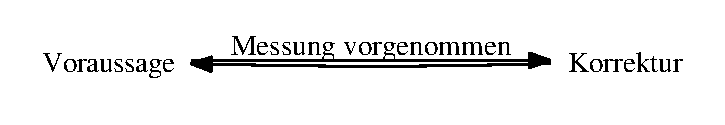
\includegraphics[width=0.5\textwidth]{kalman.eps}
	\caption{Prinzipielle Vorgehensweise eines Kalman-Filters}
	\label{fig:kalman}
\end{figure}

Das Kalman-Filter ist ein rekursiv arbeitender Filter, der für ein gegebenes System den nachfolgenden (diskreten) Systemzustand unter Berücksichtigung von normalverteilten Fehlern voraussagt. Dabei wird angenommen, dass die Veränderung des Systemzustands linear und a-priori bekannt ist~\cite{Welch1995}. Seien die Messwerte m durch Vektoren dargestellt. Dann sei $X_k$ der Zustand des Systems zum Zeitpunkt $t_k, X_k \in R^m$. Die einzelnen Systemzustände sind diskret, d.h. $t_k = t_0 + k \cdot \delta t$. Der aktuelle Systemzustand $X_k$ lässt sich mit Hilfe des vorangegangenen Zustands $X_{k-1}$ durch folgende lineare Gleichung modellieren:
\[
	X_k = F_{k-1} \cdot X_{k-1} + B_{k-1} \cdot u_{k-1} + w_{k-1}
\]
Dabei ist $F_{k-1}$ die Zustandsübergangsmatrix, $B_{k-1}$ die Dynamik der Störung (ebenfalls modelliert über eine Matrix), $u_{k-1}$ eine deterministische Störung und $w_{k-1}$ ein zufälliges Rauschen. Die einzelnen $w_i$ sind eine stochastische Größe, modelliert durch eine Normalverteilung mit dem Mittelwert 0 und der Kovarianzmatrix $Q_i$. Die einzelnen $\sum_{k=0}^k~X_k$ bilden einen stochastischen Prozess (eine sogenannte Markov-Kette). Dabei hängt das aktuelle $X_k$ nur von seinem Vorgänger $X_{k-1}$ ab (Markov-Modell erster Ordnung).

Die $X_k$ sind nicht direkt bekannt, sondern werden, wie zuvor erwähnt, durch eine (fehlerbehaftete) Messung ermittelt. Sei $Z_k$ die Messung des Systemzustands zum Zeitpunkt $t_k, Z_k \in R^m$. Der Zusammenhang zwischen dem Systemzustand und der Messung wird durch die lineare Gleichung:
\[
	Z_k = H_k \cdot X_{k-1} + v_k
\]

modelliert. Dabei ist $H_k$ die Beobachtungsmatrix und die $v_k$ eine stochastische Größe modelliert durch eine Normalverteilung mit Mittelwert 0 und der Kovarianzmatrix $R_i$. Die $v_i$ sind dabei unabhängig von den $w_i$ (Hidden-Markov-Model~\cite{MarslandBook}). 

Für die Zufallsvariable $Z_k$ nimmt man konkrete Messungen vor, mit denen sich der Systemzustand $\widehat{X}_k$ zum Zeitpunkt $t_k, \widehat{X}_k \in R^m$ schätzen lässt. Das $\widehat{X}_k$ ist dabei eine normalverteilte Zufallsvariable mit dem Mittelwert $\widehat{m}_k$ und der Kovarianz $\widehat{P}_k$.
Die beiden Variablen werden initial mit $\widehat{m}_0 = 0$ und $\widehat{P}_0$ mit der Einheitsmatrix initialisiert. 

% subsection kalman_filter (end)

\subsection{Partikelfilter} % (fold)
\label{sub:partikelfilter}

Das Kalman-Filter liefert in der Regel gute Ergebnisse unter Annahme von normalverteilten Fehlern (Störgrößen) und einem linearen Prozessmodell~\cite{MarslandBook}. Sobald diese Bedingungen nicht mehr vorliegen, versagt das Kalman-Filter, da die Fehlererwartung nicht mehr Gauss-verteilt ist.

Daher verfolgen Partikelfilter den Ansatz die aktuelle unbekannte Wahrscheinlichkeitsverteilung zu schätzen, um anschließend eine Aussage über den wahrscheinlichsten Systemzustand (des dynamischen Systems) zu treffen\cite{Doucet2009}. Hierfür wird ein Schwarm sogenannter Partikel erzeugt. Jedes Partikel besteht aus einem Gewicht und einem Punkt. Initial wird jeder Schwarm über den Punkt platziert, an dem ein neues Objekt klassifiziert wurde. Der Schwarm repräsentiert als Ganzes die Wahrscheinlichkeitsdichte in einem Anfangszustand, d.h. jedes Partikel repräsentiert einen möglichen Zustand.

\begin{figure}
	\centering
	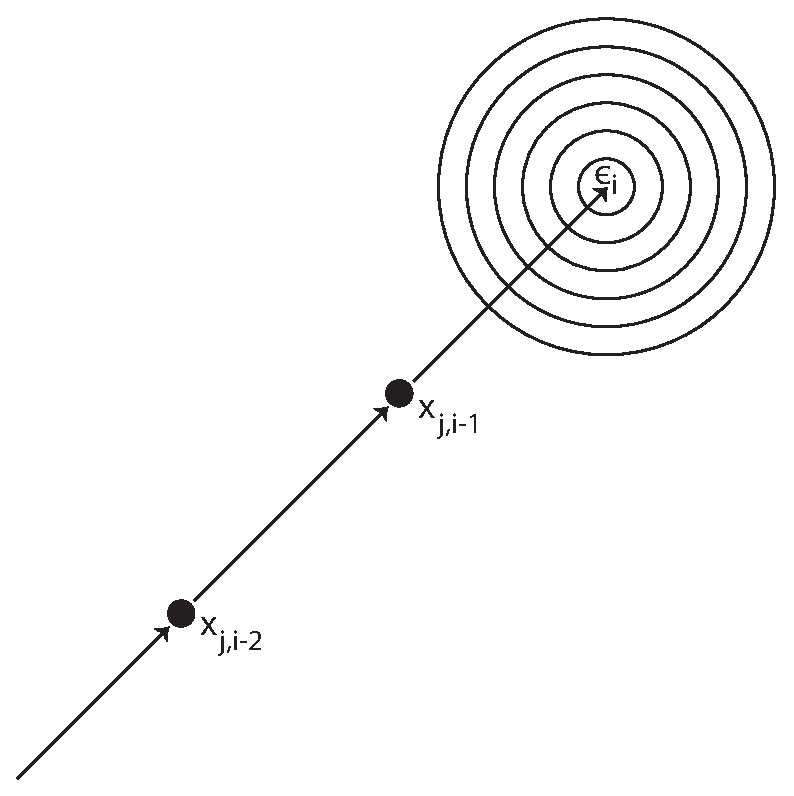
\includegraphics[width=0.5\textwidth]{bewegungsmodell.eps}
	\caption{Schematische Darstellung des Bewegungsmodells}
	\label{fig:bewegungsmodell}
\end{figure}

Um jedes Partikel anschließend neu zu platzieren, muss spezifiziert werden, wie sich ein Objekt zwischen zwei Videoframes bewegt. Dies wird über ein sogenanntes Bewegungsmodell modelliert.

\subsubsection{Bewegungsmodell} % (fold)
\label{ssub:bewegungsmodell}

Der nächste Zustand $x_t$ eines Systems lässt sich als Funktion definieren, die anhand vorheriger Zustände und einem Rauschen $\epsilon$ (Zufallsvariable) den aktuellen Zustand schätzt:
\[
	x_t = f(x_{t-1}, x_{t-2}, \ldots, x_{t-p}, \epsilon_t)
\]

Der Vorteil hierbei ist, dass sowohl die Geschwindigkeit, als auch die Beschleunigung des Objekts in die aktuelle Zustandsschätzung miteinbezogen werden. 
Werden lediglich die letzten beiden Zustände (plus einem zufälligen Rauschen) berücksichtigt, bezeichnet man das als \emph{second-order linear autoregressive model}.
Sei $x_j$ nun die Position des aktuellen Objekts und $i$ der Frameindex eines Videos, dann wird, wie in Abbildung~\ref{fig:bewegungsmodell} zu sehen, das zufällig gewählte Rauschen $\epsilon_i$ als multivariate Gaussverteilung aufgefasst.

% subsubsection bewegungsmodell (end)

Die Wahrscheinlichkeit eines Objekts an einem bestimmten Ort wird über ein sog. \emph{Erscheinungsmodell} modelliert.

\subsubsection{Erscheinungsmodell} % (fold)
\label{ssub:erscheinungsmodell}

Wenn ein neues Objekt klassifiziert wurde, wird für dieses Objekt ein sog. HSV-Farbhistogramm gespeichert. Dabei wird das HSV-Farbmodell zugrunde gelegt, um die Farbinformationen im Bild von dem Hellwert isoliert betrachten zu können.~\cite{HueVermaak2002}. Mit Hilfe des Histogramms lässt sich für jeden weiteren Frame die Wahrscheinlichkeit des Objekts an einem bestimmten Ort berechnen, in dem das ursprünglich gespeicherte Histogramm mit dem aktuellen verglichen wird.

% subsubsection erscheinungsmodell (end)

Die generelle Arbeitsweise eines Partikelfilters sieht nun wie folgt aus (vgl. Abbildung~\ref{fig:pfiltervisualisierung}):

 \begin{figure}
	\centering
	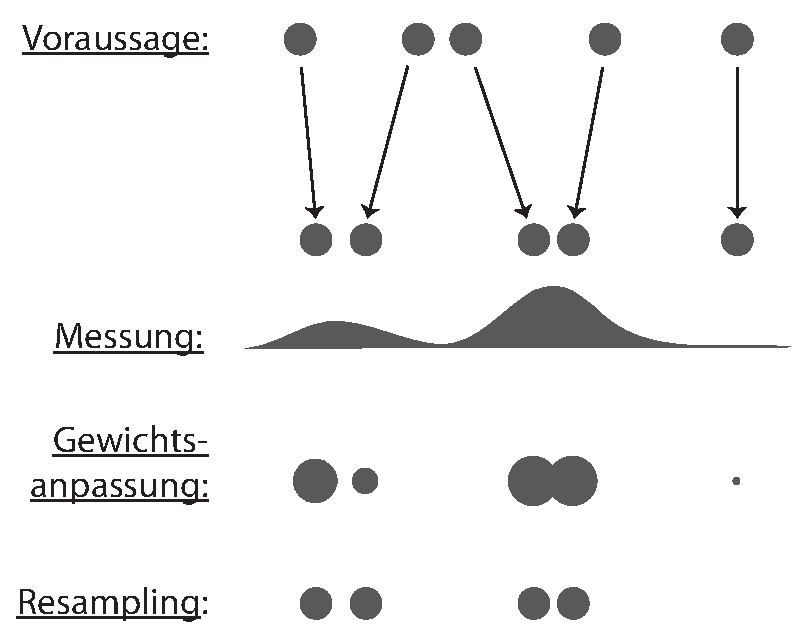
\includegraphics[width=0.5\textwidth]{pfvis.eps}
	\caption{Vorgehensweise eines Partikelfilters}
	\label{fig:pfiltervisualisierung}
\end{figure}

Zuerst wird anhand des Bewegungs- und Erscheinungsmodells jedes Partikel neu platziert. Anschließend folgt die Messung, d.h. der aktuelle Frame des Videos wird verarbeitet. Auf Grundlage dieser Messung wird für jedes Partikel das spezifische Gewicht angepass und die Summe aller Gewichte wird auf eins normalisiert. Anschließend folgt noch ein sog. \emph{Resampling} aller Partikel. Dieses Resampling vermeidet die Entartung einzelner Gewichte. Ohne diese Anpassung würde das Partikel mit dem höchsten Gewicht im Laufe der Zeit gegen eins konvergieren, wohingegen das jeweilige Gewicht der übrigen Partikel gegen null konvergieren würde. Das Resampling entfernt Partikel mit einem geringen Gewicht und dupliziert diejenigen Partikel, deren Gewicht einen bestimmten Schwellwert übersteigt.

% subsection partikelfilter (end)

\section{Gesichtserkennung und Tracking} % (fold)
\label{sec:gesichtserkennung_und_tracking}

Zur Gesichtserkennung wird ein bereits trainierter Viola-Jones Klassifikator eingesetzt (vgl.~\cite{aliMultipleHuman}). Der Gesichtsklassifikator wird dabei auf zwei verschiedene Arten eingesetzt: Einmal als sog. \emph{sliding window}, welches über das gesamte Videobild fährt, um Gesichter zu klassifizieren und einmal als Validator für zuvor klassifizierte Gesichter.

Der gesamte Ablauf des Trackings vollzieht sich wie folgt:
Im ersten Schritt wird ein Video frameweise eingelesen. Im ersten Frame des Videobilds wird der Gesichtsklassifikator verwendet, um Personen anhand ihres Gesichts im Videobild zu klassifizieren. Für jede erfolgreiche Klassifikation wird ein Bewegungspfad an der Position initialisiert, an der das Gesicht entdeckt wurde. Zudem wird für jeden Bewegungspfad ein Ausschlusszähler mit null initialisiert, der hochgezählt wird, sobald in einem nachfolgenden Frame dieses Gesicht nicht mehr klassifiziert werden konnte. Für jede Region rund um ein klassifiziertes Gesicht wird ein neues Erscheinungsmodell erstellt und ebenfalls gespeichert.

Für jeden weiteren Frame des Videobilds wird für jeden Bewegungspfad anhand eines (\emph{second-order linear autoregressive}) Bewegungsmodells die Wahrscheinlichkeitsverteilung für den Partikelschwarm bestimmt. Anhand des Farbhistogramms aus dem Erscheinungsmodells wird die spezifische Wahrscheinlichkeit für jedes Partikel ausgerechnet. Danach erfolgt ein Resampling aller Partikel. Schließlich wird, wie zuvor erwähnt, der Gesichtsklassifikator auf alle Regionen angewendet, in dem sich klassifizierte Gesichter befinden. Falls in einer Region ein Gesicht wieder zugeordnet werden kann, wird der Ausschlusszähler des dazugehörigen Bewegungspfads wieder auf null gesetzt. Falls kein Gesicht in der ausgewählten Region klassifiziert werden kann, wird der Ausschlusszähler um eins erhöht. Falls der Ausschlusszähler einen bestimmten Schwellwert überschreitet, wird der Bewegungsfpad gelöscht und aus der Menge der klassifizierten Personen genommen, da dann davon auszugehen ist, dass die betreffende Person entweder aus dem Videobild gegangen, oder komplett hinter einer Person bzw. einem Gebäude verschwunden ist.

Im letzten Schritt wird der Gesichtsklassifikator benutzt, um im kompletten Videobild nach noch nicht klassifizierten Gesichtern zu suchen. Dabei wird für jedes klassifizierte Gesicht der euklidische Abstand zwischen dem klassifiziertem Gesicht und allen Positionen aller Bewegungspfade ausgerechnet. Überschreitet die berechnete Distanz einen gewählten Schwellwert, wird davon ausgegangen, dass dieses (neue) Gesicht noch keinem Bewegungspfad zugeordnet wurde und es wird ein neuer Bewegungspfad mit der Position des entdeckten Gesichts initialisiert (ein sog. \emph{confirmation-by-classification}~Verfahren, vgl.\cite{aliMultipleHuman}).

% section gesichtserkennung_und_tracking (end)

\section{Implementierung} % (fold)
\label{sec:implementierung}

Der Quelltext\footnote{http://tinyurl.com/acivs2009} zu dieser Arbeit entstand unter Vorlage der Originalarbeit (vgl.~\cite{aliMultipleHuman}). Für die Verarbeitung des Videos wurde die freie Programmbibliothek OpenCV\footnote{http://opencv.willowgarage.com/wiki/} in der Version 2.4 und die GNU GSL Library\footnote{http://www.gnu.org/software/gsl/} verwendet.
Für das Training des Viola-Jones Klassifikators wurden 4325 Gesichter aus Videos unterschiedlicher Orte ausgeschnitten und auf die Größe von 20x20 Pixel skaliert. Des Weiteren wurden 2200 Negativbilder benutzt, um den Klassifikator zu trainieren.

Zur Gesichtsklassifikation im Video wird jeder Frame des Videos in ein Graustufenbild umgewandelt und um den Klassifikationsprozess zu beschleunigen auf 90\% der ursprünglichen Größe herunterskaliert. Anschließend erfolgt ein Histogrammausgleich des Bildes. Anschließend wird die max. Anzahl an Gesichtern im Bild ermittelt. Für jedes erkannte Gesicht wird die Region rund um das Gesicht (bzw. die Rechteckkoordinaten) gespeichert.

Danach erfolgt die Initialisierung des Trackers. Für das Tracking wird der aktuelle Frame in das HSV-Farbschema konvertiert und der Partikelfilter mit einer vorgegebenen Anzahl von 20 Partikel pro Objekt initialisiert. Für jedes zuvor erkannte Gesicht wird ein Bewegungspfad initialisiert. Jeder Bewegungspfad erhält die ID des aktuellen Frames, in welchem er initialisiert wurde, sowie ein Ausschlusszähler, der mit eins initialisiert wird, ein Histogramm der entsprechenden Region um das Gesicht und die Koordinaten des dazugehörigen Partikelzentrums.

Für die Verfolgung der Gesichter wird anschließend jeder weitere Frame zuerst in das HSV-Farbschema umgewandelt und danach für alle Bewegungspfade die Partikel und Gewichte aktualisiert. Anschließend erfolgt das Resampling des Partikelfilters. In jedem Frame wird nun erneut nach Gesichtern gesucht. Jedes erkannte Gesicht wird entweder dem dazugehörigen Bewegungspfad zugeordnet, sofern der Abstand zwischen erkanntem Gesicht im Bild und Bewegungspfad ein Maximum nicht überschreitet oder ein neuer Bewegungspfad initialisiert. Falls für bestimmte Bewegungspfade die dazugehörigen Gesichter nicht mehr erkannt wurden, wird das Gewicht für diesen Bewegungspfad um einen konstanten Wert (hier 0.5) erniedrigt. Falls das Gewicht eines Bewegungspfad kleiner -3 wird, dann wird dieser Bewegungspfad komplett aus dem Tracking genommen.

% section implementierung (end)

\section{Evaluation} % (fold)
\label{sec:evaluation}

Für die Evaluation wurde ein Video aus der Münchener Fußgängerzone\footnote{http://www.youtube.com/watch?v=TdFvJ5ye7J8} verwendet. Ein Beispielbild aus dem Video ist in Abbildung~\ref{fig:fussgaenger_muenchen} zu sehen.

\begin{figure}[tb]
	\begin{center}
		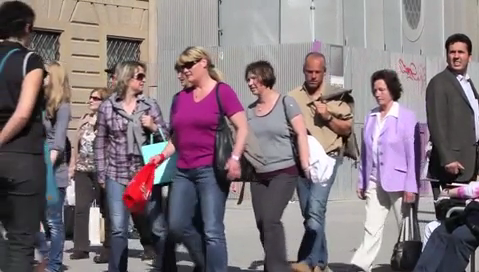
\includegraphics[width=0.49\textwidth]{fussgaenger1.png}
	\end{center}
	\caption{Beispielbild aus der Münchener Fußgängerzone}
	\label{fig:fussgaenger_muenchen}
\end{figure}
	
Das Video hat eine Auflösung von 480x272 Pixeln und eine Länge von insgesamt 29 Sekunden. Eine manuelle Auswertung ergab, dass sich insgesamt 48 verschiedene Personen durch das Bild bewegen. Während des Videos befinden sich maximal 16 Personen gleichzeitig im Videobild. 

\begin{figure*}[t]
	\subfigure[Automatisches Tracking]{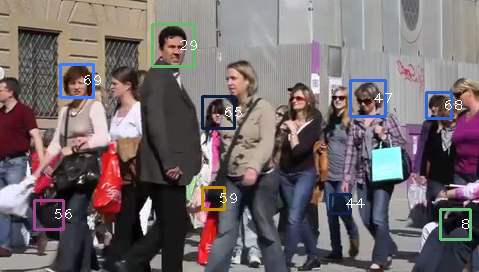
\includegraphics[width=0.49\textwidth]{maxAnzahlFussgaengerAuto.png}}\hfill
	\subfigure[Manuelle Auswertung]{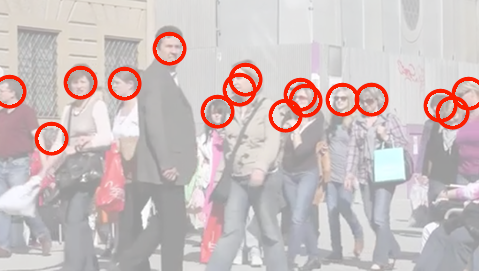
\includegraphics[width=0.49\textwidth]{maxAnzahlFussgaengerHand.png}}
	\caption{Vergleich von automatischem Tracking und manueller Auswertung bei maximaler Anzahl an Personen im Videobild}
	\label{fig:maxanzahl_fussgaenger}
\end{figure*}

In einer Stichprobe klassifiziert der verwendete Algorithmus zum belebtesten Zeitpunkt des Videos insgesamt 9 Objekte (vgl. Abbildung~\ref{fig:maxanzahl_fussgaenger}). Dabei sind lediglich 5 Objekte tatsächlich Gesichter von Personen, während die übrigen Treffer Fehlklassifikationen sind. Eine manuelle Auswertung ergibt eine tatsächliche Anzahl von 16 Personen im Bild, wobei davon 6 Personen teilweise bzw. ganz verdeckt sind. Das ergibt eine Trefferquote von 31.25\%. Insgesamt zeigt sich aber ein positiveres Bild: Der Algorithmus klassifiziert über die gesamte Videodauer insgesamt 39 von 48 unterschiedliche Personen. Das ergibt eine Trefferquote von 81.25\%. Dabei wurde das Tracking, wie in ~Abbildung \ref{fig:unterbrechung_tracking} zu sehen, von zuvor klassifizierten Personen teilweise über einige Frames hinweg unterbrochen und anschließend wieder erfolgreich aufgenommen.

\begin{figure*}[tb]
	\subfigure[Tracking einer Person mit der ID 2 im Frame 3]{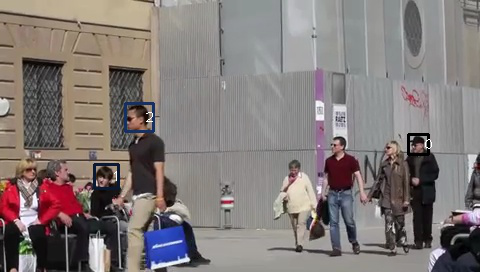
\includegraphics[width=0.32\textwidth]{frame3.png}}
	\subfigure[Verlust der Person mit der ID 2 im Frame 5]{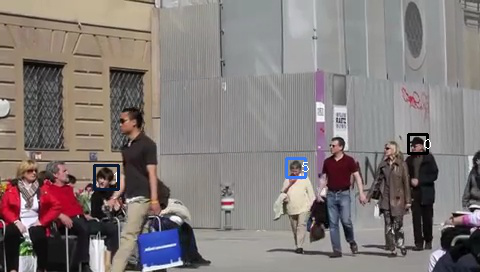
\includegraphics[width=0.32\textwidth]{frame5.png}}
	\subfigure[Wiederaufnahme der Person mit der ID 2 im Frame 7]{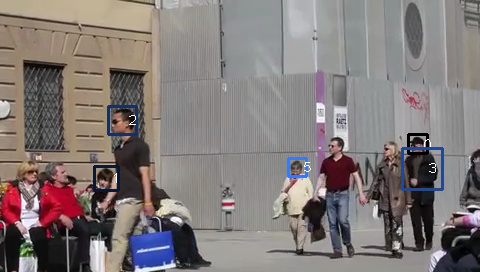
\includegraphics[width=0.32\textwidth]{frame7.png}}
	\caption{Unterbrechung des Trackings und Wiederaufnahme}
	\label{fig:unterbrechung_tracking}
\end{figure*}

Bei einigen Personen im Videobild hielt die Unterbrechung des Tracking-Vorgangs über 7 Frames an, so dass diese anschließend in einem späteren Frame bei der Gesichtsklassifizierung über das gesamte Videobild hinweg als neue Person eingestuft wurden und somit eine neue ID inklusive neuem Bewegungspfad erhielten. Neun Personen wurden in dem Video zu keiner Zeit klassifiziert. Insgesamt trackte der verwendete Algorithmus, wie in Abbildung~\ref{fig:maxanzahl_tracking} zu sehen, maximal 12 Objekte gleichzeitig, wovon 6 Objekte auch tatsächlich Personen gewesen sind.

\begin{figure}[h]
	\begin{center}
		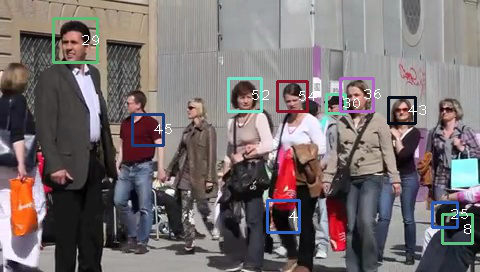
\includegraphics[width=0.49\textwidth]{maxAnzahlFussgaengerTotal.png}
	\end{center}
	\caption{Maximale Anzahl gleichzeitig getrackter Objekte}
	\label{fig:maxanzahl_tracking}
\end{figure}

% section evaluation (end)

\section{Fazit und Ausblick} % (fold)
\label{sec:fazit_und_ausblick}

Das vollständige und automatisierte Tracking aller Personen in einem Videobild stellt immer noch eine große Herausforderung aus den Bereichen Machine Learning und Computer Vision dar. Es zeigt sich, dass der verwendete Algorithmus unter idealen Bedingungen gute Ergebnisse liefert. Dabei stellt die Blickrichtung der Person, sofern diese nicht völlig abgewandt zur Kamera steht, keine Probleme dar. Die teilweise Verdeckung des Gesichts hingegen, zum Beispiel durch andere Personen, Gegenstände, Gebäude oder Hände verschlechtert die Erkennungsrate deutlich. Die evaluaierte Trefferquote von 76.8\% in der Originalarbeit (vgl.~\cite{aliMultipleHuman}) konnte in dieser Arbeit bestätigt werden.

Eine neuere Veröffentlichung aus dem Jahr 2010 beschreibt die robuste Klassifizierung von Personen in belebten Umgebungen mit Hilfe eines Histogram of Oriented Gradients-Verfahren (HOG-Verfahren) und Support-Vektor-Maschinen (\cite{Takahashi:2010}). Das HOG-Verfahren hat den Vorteil weitestgehend invariant bezüglich der Beleuchtung, Rotation und Rauschen zu sein, was es als Verfahren zur Gesichtserkennung sehr nützlich macht und weniger sog. \emph{false-positives} Erkennungen verursacht, als vergleichbare Verfahren. In dieser Arbeit wurde gezeigt, dass spezifisches Verhalten wie Rennen oder das Treffen anderer Personen selbst in belebten Umgebungen stabil erkannt werden konnte.

% section fazit_und_ausblick (end)

\bibliographystyle{apalike}
\bibliography{/Users/kai/Documents/library}

\end{document}